% Opsætter KU Tex dokument
%%%%%%%%%%%%%%%%%%%%%%%%%%%%%%%%%%%%%%%%%%%%%%%%%%%%%%%%%%%%%%%%%%%%%%%%%%%%%%%%
\documentclass{article}                                                        %
\usepackage[a4paper, hmargin={2.8cm, 2.8cm}, vmargin={2.5cm, 2.5cm}]{geometry} %
\usepackage{eso-pic}  % \AddToShipoutPicture                                   %
\usepackage{graphicx} % \includegraphics                                       %
\usepackage{subfig}                                                            %
%%%%%%%%%%%%%%%%%%%%%%%%%%%%%%%%%%%%%%%%%%%%%%%%%%%%%%%%%%%%%%%%%%%%%%%%%%%%%%%%

% Pakker til skrifttyper, tekst osv.
%%%%%%%%%%%%%%%%%%%%%%%%%%%%%%%%%%%%%%%%%%%%%%%%%%%%%%%%%%%%%%%%%%%%%%%%%%%%%%%%
    \usepackage[utf8]{inputenc}  % Implementere Unicode                        %
    \usepackage[T1]{fontenc}     % Unicode skrifttype fx. é skrives som 1 tegn %
   %\usepackage[english]{babel}  % Engelsk Ordbog                              %
    \usepackage[danish]{babel}   % Dansk Ordbog                                %
    \usepackage{microtype}       % Forbedre linjeombrydningen                  %
    \usepackage{libertine}       % Skrifttype                                  %
%%%%%%%%%%%%%%%%%%%%%%%%%%%%%%%%%%%%%%%%%%%%%%%%%%%%%%%%%%%%%%%%%%%%%%%%%%%%%%%%

% Pakker til matematik og kode.
%%%%%%%%%%%%%%%%%%%%%%%%%%%%%%%%%%%%%%%%%%%%%%%%%%%%%%%%%%%%%%%%%%%%%%%%%%%%%%%%
    \usepackage{mathtools}       % Udvidelse til amsmath pakken                %
    \usepackage{amsthm}          % Pakke til bevisførelse                      %
    \usepackage{amssymb}         % Extra matematiske symboler                  %
%%%%%%%%%%%%%%%%%%%%%%%%%%%%%%%%%%%%%%%%%%%%%%%%%%%%%%%%%%%%%%%%%%%%%%%%%%%%%%%%

% Pakker til layout.
%%%%%%%%%%%%%%%%%%%%%%%%%%%%%%%%%%%%%%%%%%%%%%%%%%%%%%%%%%%%%%%%%%%%%%%%%%%%%%%%
    \usepackage{fancyhdr}            % Gør det muligt at bruge sidehoveder     %
    \usepackage{graphicx}            % Mulighed for bl.a. \includegraphics     %
    \usepackage{colortbl}            % Hvis man vil farvelægge sine tabeller   %
    \usepackage{array}               % Gør miljøerne array og tabular bedre    %
    \usepackage{parskip}             % Første paragraf i afsnit indrykkes ikke %
    \usepackage{titlesec}            % Tilpassing af afstand mellem sektioner  %
    \usepackage[lastpage,user]{zref} % Side x af y                             %
%%%%%%%%%%%%%%%%%%%%%%%%%%%%%%%%%%%%%%%%%%%%%%%%%%%%%%%%%%%%%%%%%%%%%%%%%%%%%%%%


% Implementerer en række makroer og de pakker der er importeret
%%%%%%%%%%%%%%%%%%%%%%%%%%%%%%%%%%%%%%%%%%%%%%%%%%%%%%%%%%%%%%%%%%%%%%%%%%%%%%%%
    \pagestyle{fancy}                        % Implementerer sidehoved         %
    \lhead{Gymnasietjenesten}                % Venstre sidehoved               %
    \rhead{DIKU}                             % Højre sidehoved                 %
    \cfoot{\thepage\ of \zpageref{LastPage}} % Side x af y                     %
    \newtheorem*{prp}{Propostion}            % Skaber nyt theorem              %
%%%%%%%%%%%%%%%%%%%%%%%%%%%%%%%%%%%%%%%%%%%%%%%%%%%%%%%%%%%%%%%%%%%%%%%%%%%%%%%%

% Mindsker afstanden mellem sektioner
%%%%%%%%%%%%%%%%%%%%%%%%%%%%%%%%%%%%%%%%%%%%%%%%%%%%%%%%%%%%%%%%%%%%%%%%%%%%%%%%%%
\titlespacing\section{0pt}{12pt plus 4pt minus 2pt}{0pt plus 1pt minus 3pt}      %
\titlespacing\subsection{0pt}{12pt plus 4pt minus 2pt}{0pt plus 1pt minus 3pt}   %
\titlespacing\subsubsection{0pt}{12pt plus 4pt minus 2pt}{0pt plus 1pt minus 3pt}%
%%%%%%%%%%%%%%%%%%%%%%%%%%%%%%%%%%%%%%%%%%%%%%%%%%%%%%%%%%%%%%%%%%%%%%%%%%%%%%%%%%

% Laver titel
%%%%%%%%%%%%%%%%%%%%%%%%%%%%%%%%%%%%%%%%%%%%%%%%%%%%%%%%%%%%%%%%%%%%%%%%%%%%%%%%
    \title{                                                                    %
      \vspace{13em}                                                            %
      \Large{Datalogisk Institut Københavns Universitet} \\                    %
      \Huge{Oplæg til SRP og SOP}                %
    }                                                                          %
                                                                               %
    \author{                                                                   %
      \Large{Arinbjørn Brandsson} - \texttt{Arbr@di.ku.dk} \\                  %
      \Large{Benjamin Rotendahl} - \texttt{Bero@di.ku.dk} \\                   %
    }                                                                          %
                                                                               %
    \date{                                                                     %
        \vspace{22em}                                                          %
        \today                                                                 %
    }                                                                          %
%%%%%%%%%%%%%%%%%%%%%%%%%%%%%%%%%%%%%%%%%%%%%%%%%%%%%%%%%%%%%%%%%%%%%%%%%%%%%%%%

%%%%%%%%%%%%%%%%%%%%%%%%%%%%%%%%%%%%%%%%%%%%%%%%%%%%%%%%%%%%%%%%%%%%%%%%%%%%%%%%
%%%%%%%%%%%%%%%%%%%%      Her starter dokumentet    %%%%%%%%%%%%%%%%%%%%%%%%%%%%
\begin{document}

% KU forside
%%%%%%%%%%%%%%%%%%%%%%%%%%%%%%%%%%%%%%%%%%%%%%%%%%%%%%%%%%%%%%%%%%%%%%%%%%%%%%%%%
    \AddToShipoutPicture*{\put(0,0){\includegraphics*[viewport=0 0 700 600]     %
    {include/ku-farve}}}                                                        %
    \AddToShipoutPicture*{\put(0,602){\includegraphics*[viewport=0 600 700 1600]%
    {include/natbio-farve}}}                                                    %
    \AddToShipoutPicture*{\put(0,0){\includegraphics*{include/nat-en}}}         %
    \clearpage                                                                  %
%%%%%%%%%%%%%%%%%%%%%%%%%%%%%%%%%%%%%%%%%%%%%%%%%%%%%%%%%%%%%%%%%%%%%%%%%%%%%%%%%

%Disse linjer skaber forside, evt indholdsfortegnelse, og sætter sidetal
%%%%%%%%%%%%%%%%%%%%%%%%%%%%%%%%%%%%%%%%%%%%%%%%%%%%%%%%%%%%%%%%%%%%%%%%%%%%%%%%
    \maketitle              % Forside
    \thispagestyle{empty}   % Fjerner sidetal forside

        % Slå disse til hvis der ønskes indholdsfortegnelse
        %%%%%%%%%%%%%%%%%%%%%%%%%%%%%%%%%%%%%%%%%%%%%%%%%%%%%%%%%%%%%%%%%%%%%%%%
        %    \newpage                % Side til indholdsfortegnelse            %
        %    \thispagestyle{empty}   % Fjerner sidetal fra indholdsfortegnelse %
        %    \tableofcontents        % Skaber indholdsfortegnelse              %
        %%%%%%%%%%%%%%%%%%%%%%%%%%%%%%%%%%%%%%%%%%%%%%%%%%%%%%%%%%%%%%%%%%%%%%%%
    \newpage                % Første rigtige side
    \setcounter{page}{1}    % Sætter rigtigt sidetal på første side
%%%%%%%%%%%%%%%%%%%%%%%%%%%%%%%%%%%%%%%%%%%%%%%%%%%%%%%%%%%%%%%%%%%%%%%%%%%%%
\section{Oplæg til SRP/SOP}
    Onsdag den 18/10 afholder Gymnasietjenesten på DIKU en serie af oplæg man
    kan bruge som indspark til sit projekt. Skriver man for eksempel i
    Virksomhedsøkonomi og informatik vil man kunne få en forklaring af hvordan
    bitcoins fungerer. Den viden man få ved oplæggene kan så indrages i ens
    projekt og man vil kunne få svar på de spørgsmål man måtte have om ens emne.
    Oplæggenes sværhedsgrad er rettet mod gymnasieelever i 3.G.



\section{Praktisk information}
    Workshoppen finder sted i HCØ bygningen, hvor der vil være forelæsning i
    auditorium 10 og øvelser i de omliggende  lokaler.

    Adressen er Universitetsparken 5, 2100 København.
    Op til kl 10.00 vil der være en til at tage imod, og vise jer hen til
    auditoriet ved indgangen markeret på kortet.
    \begin{figure}[h!]
        \caption{Hovedindgang til HCØ}
        \centering
        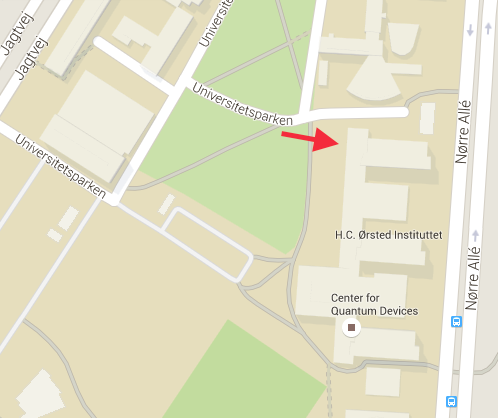
\includegraphics[width=0.5\textwidth]{./include/kort.png}
    \end{figure}

    \subsection{Program for mandag}
    \begin{description}
        \item[kl 10.00-12.00] | Velkomst og forelæsning ~ \\
        Vi starter med velkomst og en forelæsning om LaTeX.
        Forelæsningen vil give en introduktion til hvad LaTeX er, hvordan det
        fungerer, og hvilke fordele det har over programmer som Word.

        \item[kl 12.00-12.45] | Pause ~ \\
        Til frokost kan i enten have madpakke med, eller tage penge med til
        kantinen.

        \item[12.45 - 15.00] | Øvelser ~ \\
        Til øvelserne vil i blive givet et print lavet i LaTeX med forskellige
        formler, tabeller, og figurer. Jeres opgave vil så være at genskabe
        dette dokument i LaTeX. Vi samler op med en gennemgang på projektoren.
    \end{description}

    \subsection{Program for tirsdag}
    \begin{description}
        \item[kl 10.00-12.00] | Opsamling fra mandag og øvelser ~ \\
        Tirsdag vil vi starte med at vise, hvordan LaTeX brillerer særligt
        ved større rapporter. Herefter vil vi gerne bede jer om at tage en af
        jeres egne afleveringer med, som i så skal ``TeXe''.

        \item[kl 12.00-12.45] | Pause ~ \\
        Til frokost kan i enten have madpakke med, eller tage penge med til
        kantinen.

        \item[12.45 - 15.00] | Intro til databehandling ~ \\
        Vi vil holde en forelæsning, hvor vi demonstrerer forskellige
        databehandlings værktøjer, samt hvordan de sammenarbejder med LaTeX.
    \end{description}

\section{Installationsguide}
    Det kræver to programmer at køre LaTeX.
    Det ene program er selve LaTeX-``motoren'' der bygger pdf'en.
    Det andet program er en LaTeX editor, hvori man skriver filen, som LaTeX
    skal bygge fra.

    \subsection{LaTeX-motor}
    Følg disse trin for at installere LaTeX-motoren.

    \begin{itemize}
        \item Download installationsfilen
        \footnote{Vi anbefaler at man tager en kop kaffe mens den downloades}.\\
        Mac-brugere skal hente denne installations fil
        \begin{quote}
         http://tug.org/cgi-bin/mactex-download/MacTeX.pkg
        \end{quote}

        Windows-brugere skal hente denne lille fil, som så henter en stor fil
        ned.
        \begin{quote}
        http://mirror.ctan.org/systems/texlive/tlnet/install-tl-windows.exe
        \end{quote}

        \item Dobbeltklik den downloadede fil, således at disse nedenstående
        vinduer åbner.
		\begin{figure}[h]
    		\centering
    		\subfloat[Mac brugere]{
                {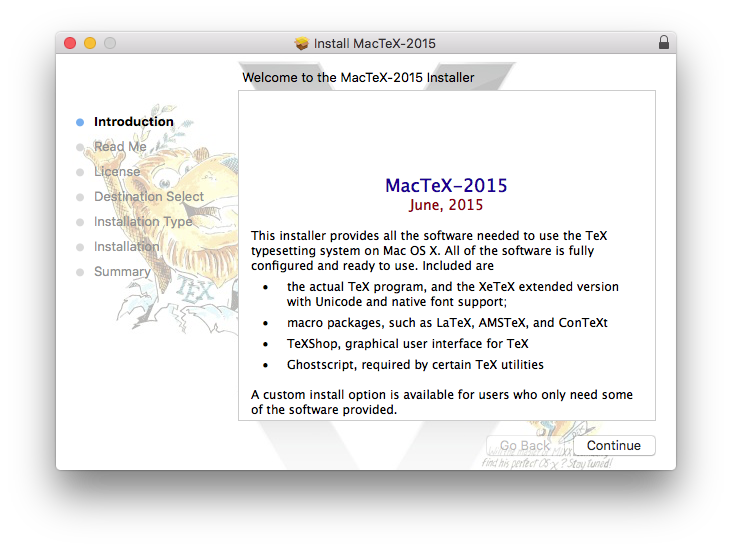
\includegraphics[width=6cm]{./include/mac1.png}}}%
	    	\qquad
	    	\subfloat[Windows brugere]{{
                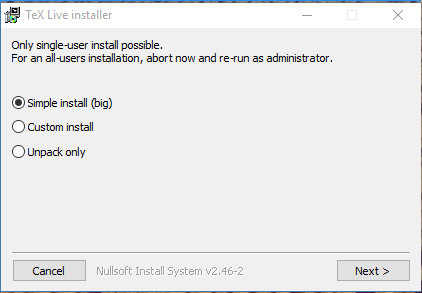
\includegraphics[width=6cm]{./include/windows1.png}}}%
		    \caption{Installations vinduerne}%
		\end{figure}\\
        Mac brugere skal forsætte med at trykke på ``continue'' indtil programmet
        er installeret.


        Windows brugere skal vælge "simple install" og trykke ``next''.
        Vær sikker på at alle indstillinger passer med dem der vises på
        nedenstående figur. Afslut installationen af din LaTeX-motor ved at
        trykke ``install''.

        \begin{figure}[h!]
            \caption{Indstillinger for windows}
            \centering
            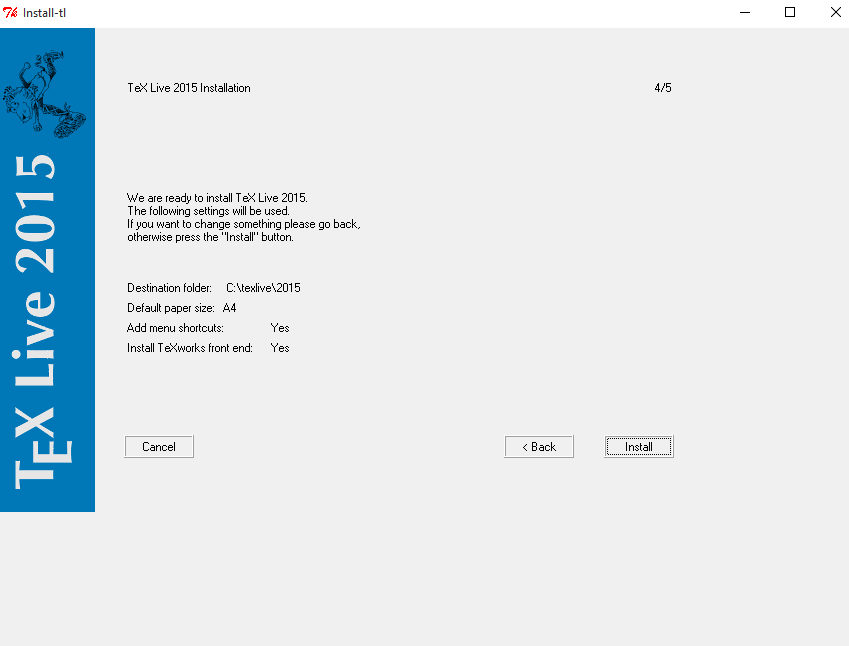
\includegraphics[width=0.6\textwidth]{./include/winSet.png}
        \end{figure}
        Du har nu installeret en tex motor.
		 \end{itemize}

        \subsection{Latex Editor}
        Det program vi bruger til at interagere med LaTeX motoren hedder
        ``TeXMaker''. Hent installationsfilen her
            \begin{quote}
            Mac : http://www.xm1math.net/texmaker/TexmakerMacosxLion.zip  \\
            Windows : http://www.xm1math.net/texmaker/texmakerwin32\_install.exe
            \end{quote}

        Mac-brugere skal udpakke zip filen ved at dobbeltklikke på den og
        flytte programmet ind i deres ``Applications'' mappe.
        Windows-brugere skal dobbeltklikke på filen og vælge install.
   		\begin{figure}%
    		\centering
    		\subfloat[Mac brugere]{
            {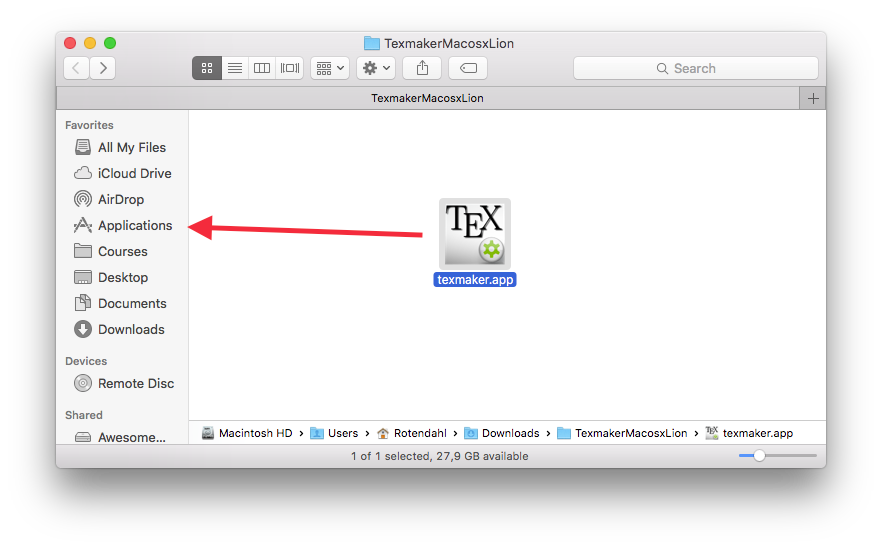
\includegraphics[width=5cm]{./include/texMove.png}}}%
	    	\qquad
	    	\subfloat[Windows brugere]{
            {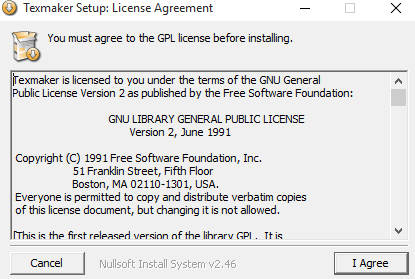
\includegraphics[width=5cm]{./include/winMove.png}}}
		\end{figure}

	I mangler nu kun at installere dansk ordbog i LaTex.
	Dette gøres ved at hente denne zip fil, og udpakke den til et passende sted
	på jeres computer.
	\begin{quote}
			http://rotendahl.dk/da-DK.zip
	\end{quote}

	Herefter går i ind i indstillingere i TexMaker, og vælger den fil i
	lige har udpakket.
	Indlæs så den danske ordbog ved at vælge den som vist i billedet.
	\begin{figure}[h!]
    	\caption{Dansk ordbog}
        \centering
        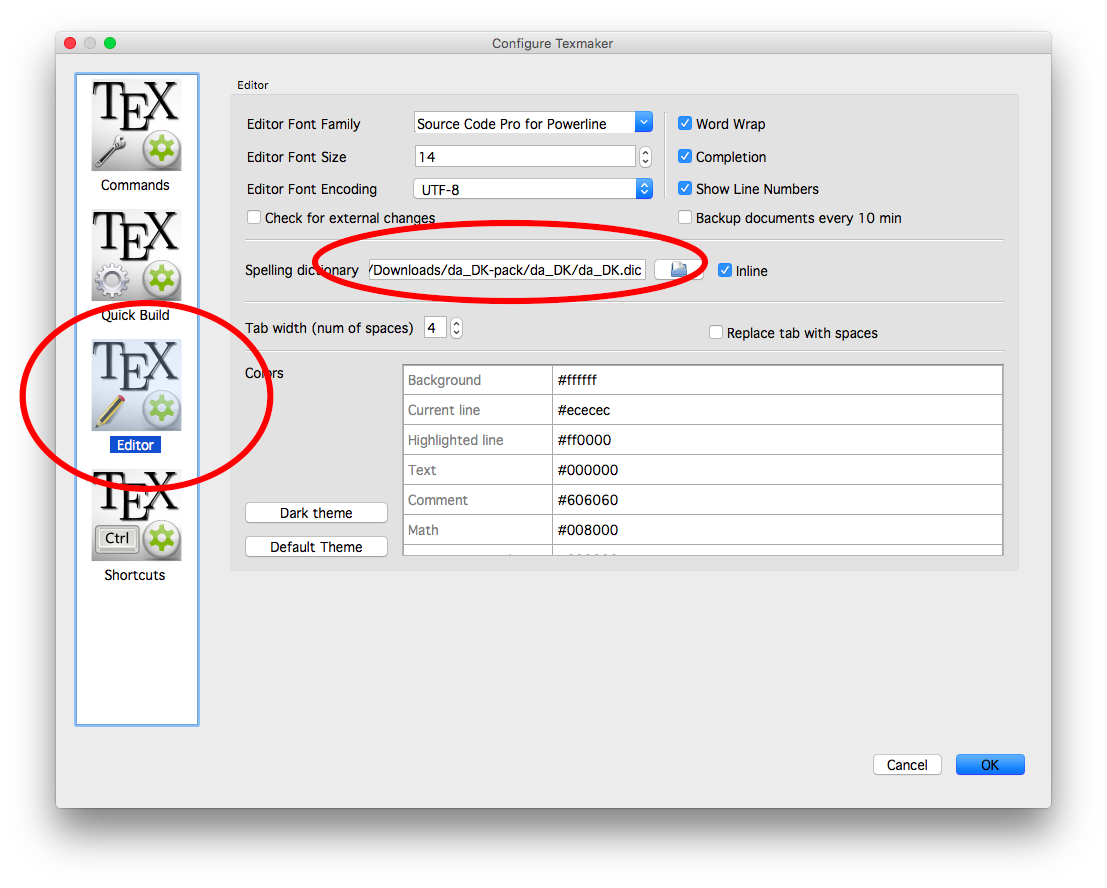
\includegraphics[width=0.6\textwidth]{./include/danish.png}
    \end{figure}

	\section{Outro}
	Du har nu installeret alt og er klar til workshoppen.
	Hvis du allerede nu er lidt nysgerrig på, hvad det som du har installeret
	kan bruges til, så kan du hente følgnede dokument og se hvordan det er
	skrevet.
    \\ Vi glæder os til at se jer den 12.!
	\begin{quote}
		http://rotendahl.dk/eks-tex.zip
	\end{quote}

\end{document}
